\documentclass[12pt, a4paper]{article}
\usepackage[utf8]{inputenc}
\usepackage[portuguese]{babel}
\usepackage{geometry}
\geometry{a4paper, margin=2.5cm}
\usepackage{amsmath, amsfonts, amssymb}
\usepackage{hyperref}
\usepackage{graphicx}
\graphicspath{{results/figures/}{../results/figures/}}
\usepackage{float}
\usepackage{placeins}

\begin{document}

% ============================================================
% CAPA
% ============================================================
\begin{titlepage}
\centering
\includegraphics[width=3cm]{logoUFS-5b7c1d387ab83d8c06b27e6943deddc28337984b1536cf0b2aad371d4db297a0.png}\\[0.8cm]
{\large UNIVERSIDADE FEDERAL DE SERGIPE}\\
{\large DEPARTAMENTO DE COMPUTAÇÃO}\\
{\large PROGRAMA DE PÓS-GRADUAÇÃO EM CIÊNCIA DA COMPUTAÇÃO}\\[2cm]

{\Large\bfseries Atividade 2 (AV2): Recuperação de Contexto e Otimização para IA Generativa}\\[3cm]

{\large Carlos Adriano Gama Cerqueira}\\
{\large Gabriel Cavalcante Silva}\\
{\large Sidney Matheus Santos de Andrade}\\
{\large Charlie Rodrigues Fonseca}\\
{\large Igor Rafael Silva Xavier}\\[2cm]

\vfill
{\large Aracaju/SE}\\
{\large \today}
\end{titlepage}

% ============================================================
% CONTRACAPA (folha de rosto)
% ============================================================
\begin{titlepage}
\centering
{\large Carlos Adriano Gama Cerqueira}\\
{\large Gabriel Cavalcante Silva}\\
{\large Sidney Matheus Santos de Andrade}\\
{\large Charlie Rodrigues Fonseca}\\
{\large Igor Rafael Silva Xavier}\\[3cm]

{\Large\bfseries Atividade 2 (AV2): Recuperação de Contexto e Otimização para IA Generativa}\\[3cm]

\begin{minipage}{0.6\textwidth}
Trabalho apresentado à disciplina de Projeto e Análise de Algoritmos (PAA), como requisito parcial de avaliação da Atividade 2 (AV2), sob orientação do(a) professor(a) Glauco de Figueiredo Carneiro.
\end{minipage}\\[3cm]

\vfill
{\large Aracaju/SE}\\
{\large \today}
\end{titlepage}

% ============================================================
% SUMÁRIO
% ============================================================
\newpage
\tableofcontents
\thispagestyle{empty}
\newpage

\setcounter{page}{1}

% ============================================================
% SEÇÕES DO TRABALHO (PACOTES 1 A 5)
% ============================================================
\section{Programação dinâmica para seleção de contexto}

\subsection{Modelo e estruturas de dados}
Foi implementado o problema da mochila 0/1 em \texttt{src/knapsack\_dp.py}. A entrada é uma lista de $n$ candidatos na ordem recebida e um orçamento inteiro $W\geq 0$. Cada candidato possui identificador único, valor finito $v_i\geq 0$ (score BM25) e custo inteiro positivo $t_i$ (\texttt{len(tokens)}). Busca-se um subconjunto que maximize a soma dos valores sem ultrapassar $W$, usando cada candidato no máximo uma vez. O ótimo é restrito aos candidatos recuperados (até $M=200$), não ao corpus inteiro, e não garante qualidade semântica ou diversidade.

A tabela \texttt{dp}, com $(n+1)\times(W+1)$ células, armazena os melhores valores por prefixo e capacidade. Um vetor guarda os candidatos reconstruídos. A função compartilhada \texttt{make\_selection} devolve identificadores crescentes, valor total, custo total e a contagem convencional de operações $n(W+1)$.

\subsection{Recorrência e pseudocódigo}
Para $0\leq w\leq W$, $dp[0][w]=0$. Para $1\leq i\leq n$:
\[
dp[i][w]=
\begin{cases}
dp[i-1][w], & t_i>w,\\
\max\{dp[i-1][w],\;dp[i-1][w-t_i]+v_i\}, & t_i\leq w.
\end{cases}
\]
O pseudocódigo usa índices de candidatos iniciados em zero:
\begin{verbatim}
solve(candidatos, W):
    validate(candidatos, W)
    n <- tamanho(candidatos)
    dp <- tabela (n+1) por (W+1) de zeros
    para i de 1 até n:
        c <- candidatos[i-1]
        para w de 0 até W:
            dp[i][w] <- dp[i-1][w]
            se c.cost <= w:
                dp[i][w] <- max(dp[i][w],
                    dp[i-1][w-c.cost] + c.value)
    escolhidos <- vetor vazio; w <- W
    para i de n até 1:
        se dp[i][w] != dp[i-1][w]:
            c <- candidatos[i-1]
            acrescentar c a escolhidos
            w <- w - c.cost
    retornar make_selection(escolhidos, n*(W+1))
\end{verbatim}
Na F7, com $W=10$, os candidatos $(id,v,t)$ são $(1,6,4)$, $(2,6,6)$ e $(3,7,5)$. Os valores $dp[i][10]$, para $i=0,1,2,3$, são $0,6,12,13$. A reconstrução retorna $[1,3]$, valor 13 e custo 9. Empates mantêm a solução do prefixo anterior, omitindo o item atual; a ordenação dos identificadores só ocorre na saída.

\subsection{Corretude}
O invariante é: $dp[i][w]$ representa o maior valor obtido usando apenas os $i$ primeiros candidatos com capacidade $w$. A prova é por indução em $i$. Na base $i=0$, somente o conjunto vazio é possível, de valor zero. Suponha correta a linha $i-1$. Uma solução ótima ou exclui o item $i$, obtendo no máximo $dp[i-1][w]$, ou o inclui, se $t_i\leq w$, obtendo no máximo $dp[i-1][w-t_i]+v_i$. Ambas as alternativas são realizáveis pela hipótese indutiva; seu máximo fornece exatamente o ótimo da célula. Logo, $dp[n][W]$ é ótimo.

Na reconstrução, se $dp[i][w]\neq dp[i-1][w]$, a inclusão do item $i$ é necessária para atingir o valor da célula, e o subproblema restante tem capacidade $w-t_i$. Caso contrário, existe uma solução ótima sem esse item. Cada passo diminui $i$, impedindo reutilização; somente itens que cabem podem ser incluídos. Assim, a reconstrução termina e retorna um subconjunto ótimo e viável. A prova pressupõe aritmética exata; na implementação, os scores usam \texttt{float}, sujeitos a arredondamento. A comparação entre células segue o contrato, sem tolerância artificial de desempate.

\subsection{Análise e limites}
No modelo RAM, com aritmética, comparações e acessos de custo unitário, a inicialização usa $\Theta((n+1)(W+1))$ operações; o preenchimento visita $n(W+1)$ células e a reconstrução custa $O(n)$. A ordenação dos $k$ escolhidos custa $O(k\log k)$, absorvido pelo preenchimento porque $k\leq\min(n,W)$ para custos inteiros positivos. Tempo e espaço são $\Theta((n+1)(W+1))$, ou $\Theta(nW)$ para $n,W\geq1$, tanto no melhor quanto no pior caso: não há interrupção antecipada. A contagem \texttt{ops} mede somente as transições, não o trabalho total.

Sem reconstrução, uma única linha atualizada por capacidades decrescentes reduz o espaço a $\Theta(W+1)$, usualmente $\Theta(W)$. O custo é pseudo-polinomial: depende do valor de $W$, cuja representação binária ocupa $\Theta(\log(W+1))$ bits para $W\geq1$. Tokenização, embeddings, disco, API e geração pelo LLM não são contabilizados pelo algoritmo.

Os testes T01 e T02 verificam F1, F7, F4, F6 e o contraexemplo F9: o DP escolhe $[2,3,4]$, de valor $9{,}1$, descartando o documento de valor individual 9,0. Portanto, ótimo aditivo não significa preservar a evidência individualmente mais relevante. Testes suplementares cobrem validação, vazios, empates, imutabilidade da entrada, uso único dos itens, 200 candidatos e comparação com enumeração exaustiva em instâncias pequenas reprodutíveis.

\subsection*{Uso de IA neste pacote}
\begin{itemize}
  \item Ferramenta/modelo: assistente do editor de texto Zed; revisão com OpenAI GPT-6.1 Sol.
  \item Finalidade e prompts: escrita dos testes automatizados e revisão da implementação do algoritmo de knapsack.
  \item Verificação: testes automatizados, comparação independente com enumeração exaustiva, Pyright e Ruff.
\end{itemize}

\section{Linhas de base gulosas}

Os três métodos desta seção são as linhas de base da programação dinâmica:
escolhem os documentos em uma única passada, sem tabela. Todos chamam
\texttt{validate}, ordenam os candidatos com o \texttt{merge\_sort} da AV1
(chave decrescente, desempate pelo menor \texttt{doc\_id}) e pegam cada
documento que ainda cabe no que sobra de $W$ (\texttt{src/knapsack\_greedy.py}).

\subsection{As três regras}

\begin{itemize}
  \item \texttt{greedy\_score} (chave $v_i$): o mais relevante primeiro; é o
    top-$k$ da AV1 respeitando $W$.
  \item \texttt{greedy\_ratio} (chave $v_i/c_i$): mais relevância por token;
    prefere documentos densos.
  \item \texttt{greedy\_ratio\_plus}: o maior entre o resultado de
    \texttt{greedy\_ratio} e o melhor documento que cabe sozinho; protege
    contra o caso em que um documento grande vale mais que o conjunto denso.
\end{itemize}

\begin{algorithm}[ht]
\caption{Gulosos: \texttt{greedy\_score} = \textsc{Guloso}$(C, W, v_i)$ e
\texttt{greedy\_ratio} = \textsc{Guloso}$(C, W, v_i/c_i)$.}
\begin{algorithmic}[1]
\Function{Guloso}{$C, W, \mathit{chave}$}
  \State $S \gets \emptyset$;\; $r \gets W$
  \For{$i \in \textsc{MergeSort}(C, \mathit{chave})$}
    \Comment{decrescente; empate pelo menor id}
    \State \textbf{se} $c_i \le r$ \textbf{então} $S \gets S \cup \{i\}$;\; $r \gets r - c_i$
  \EndFor
  \State \Return $S$
\EndFunction
\Function{RatioPlus}{$C, W$}
  \State $S \gets \textsc{Guloso}(C, W, v_i/c_i)$;\;
    $j \gets \arg\max\{v_i : c_i \le W\}$
  \State \Return o de maior valor entre $S$ e $\{j\}$ \Comment{empate: $S$}
\EndFunction
\end{algorithmic}
\end{algorithm}

\subsection{Quando é ótimo e quando é heurística}

A regra $v/c$ foi proposta por Dantzig~\cite{dantzig1957} e é ótima na
mochila fracionária, em que se pode levar parte de um
documento~\cite{cormen2012}. Argumento de troca: com os itens em ordem de razão
($r_1 \ge \dots \ge r_n$) e nem todos cabendo, o guloso $x$ enche os $k-1$
primeiros e uma fração do $k$-ésimo, usando todo o orçamento. Se uma solução
ótima $x^*$ difere de $x$, no primeiro índice $i$ em que diferem vale
$x^*_i < x_i$, e existe $j > i$ com $x^*_j > x_j$. Passar $\varepsilon$ tokens
de $j$ para $i$ mantém a viabilidade e muda o valor em
$\varepsilon(r_i - r_j) \ge 0$; repetindo, $x^*$ vira $x$ sem perder valor.

Na mochila 0/1 a troca deixa de valer. Em F1 ($W = 10$; itens
$(v, c) = (10, 10)$ e $(2, 1)$), \texttt{greedy\_ratio} pega o item 2 (razão 2
contra 1) e o item 1 deixa de caber: valor 2 contra o ótimo 10. Com o item 1
trocado por $(W, W)$, a razão entre os dois é $2/W$, que tende a zero.
\texttt{greedy\_score} falha no caso oposto: em F9 fica com o documento de
valor 9{,}0, que ocupa todo o orçamento, quando $\{2, 3, 4\}$ vale 9{,}1.
Assim, \texttt{greedy\_score} e \texttt{greedy\_ratio} não têm garantia de
aproximação.

\subsection{Garantia de 1/2 para \texttt{greedy\_ratio\_plus}}

\textbf{Teorema~\cite{kellerer2004}.} \texttt{greedy\_ratio\_plus} obtém pelo menos
$\mathrm{OPT}/2$.

\textbf{Prova.} Itens com $c_i > W$ não entram em nenhuma solução e podem ser
descartados. Se os demais cabem juntos, o guloso pega todos e é ótimo. Senão,
seja $k$ o primeiro item, em ordem de razão, que o guloso não pega. Todos os
anteriores foram pegos, então o guloso vale $G \ge \sum_{i<k} v_i$, e a solução
fracionária ótima leva esses itens e uma fração de $k$. Logo
\[
  \mathrm{OPT} \le \mathrm{OPT}_{\text{frac}} \le \sum_{i<k} v_i + v_k
  \le G + v_{\max} \le 2\max(G, v_{\max}),
\]
em que $v_{\max}$ é o maior valor de um item que cabe sozinho, e
$\max(G, v_{\max})$ é exatamente o que o método devolve. \hfill$\square$

A constante é justa: com $W = 100$ e itens $(1{,}1;\ 1)$, $(50;\ 50)$ e
$(50;\ 50)$, o método obtém 51{,}1 e o ótimo é 100.

\subsection{Análise e riscos para o contexto do LLM}

Montar os pares custa $\Theta(n)$, o \texttt{merge\_sort} faz no máximo
$n\lceil\log_2 n\rceil$ comparações~\cite{cormen2012} e a varredura (mais a busca do melhor item,
no \texttt{ratio\_plus}) custa $\Theta(n)$: tempo $\Theta(n \log n)$,
independente de $W$, e espaço $\Theta(n)$. Com $n = 200$ e $W = 2000$, a regra
de \texttt{ops} (comparações $+\ n$) dá no máximo 1.800 operações, contra
$n(W+1) = 400.200$ do DP. Custos fora do algoritmo (tokenização, índice, BM25,
disco, API e geração) não entram em \texttt{t\_selecao\_ms}.

Nenhuma regra gulosa trata redundância ou diversidade: duas notícias quase
iguais entram juntas e gastam tokens com a mesma evidência (métrica
\texttt{redundancy}). Trabalhos recentes formulam a seleção de contexto do RAG
como uma variante da mochila que penaliza redundância e apontam que a seleção
gulosa aproveita mal a janela~\cite{xu2026}. A regra $v/c$ favorece textos curtos, que podem encher a
janela de fragmentos; a regra por score favorece textos longos e pode gastar
todo o orçamento em um só documento (F9).

\subsection*{Uso de IA neste pacote}
\begin{itemize}
  \item Ferramenta e modelo: Claude (Anthropic).
  \item Finalidade: gerar rascunhos do código, dos testes T03 e T04 e desta
    seção a partir do plano da AV2. Os requisitos vieram do plano; a revisão,
    as decisões e a validação dos resultados foram do autor.
  \item Prompts relevantes (até 5): implementar o Pacote 2 do plano (gulosos);
    explicar a garantia de 1/2 e o contraexemplo F1; buscar uma referência
    clássica e uma recente para a seção.
  \item Sugestões aproveitadas, corrigidas ou rejeitadas: após revisão, foram
    aproveitadas a estrutura das três funções e a varredura completa (o guloso
    segue procurando itens menores depois de um que não cabe); a seção foi
    reduzida para caber em 2 páginas; o autor pediu a inclusão de uma
    referência clássica~\cite{dantzig1957} e uma recente~\cite{xu2026} e
    aprovou as escolhidas, além de Cormen e Kellerer.
  \item Erros identificados e como foram verificados: testes com
    \texttt{pytest}, comparação com força bruta em instâncias aleatórias e
    conferência dos exemplos F1 e F9 com as instâncias fixas do plano.
\end{itemize}

\section{Identificação, Problema Formal e Linhas de Base (Pacote 3)}
\label{sec:pacote3}

\subsection{Identificação do Trabalho, Corpus e Contribuições}
Este trabalho integra a disciplina de Projeto e Análise de Algoritmos (PAA --- 2026.2, UFS) sob o \textbf{Tema 6 (Notícias de Fontes Públicas)}. O repositório no GitHub do usuário \texttt{gabrielkavalcante} é versionado da entrega da AV1 (tag \texttt{av1}, commit \texttt{47aaffc}) até a entrega final da AV2 (tag \texttt{av2}, branch \texttt{main}), sob licença MIT para o código-fonte. O corpus é o \emph{News of the Site Folha de S.Paulo} (Kaggle, \texttt{marlesson/news-of-the-site-} \texttt{folhauol}, acessado em 09/09/2026; ficha em \texttt{docs/FICHA\_CORPUS.md}), com $167.053$ notícias em português brasileiro (jan/2015 a set/2017) sob licença \texttt{CC0: Public Domain} no Kaggle (mantidos os direitos editoriais da Folha/UOL). A amostragem reprodutível (\texttt{seed=42}) para $N \in \{10.000, 50.000\}$ resulta em $9.954$ e $49.741$ documentos reais após limpeza de textos vazios e duplicatas de título+texto, sem \emph{chunking} (mediana de $238$ e P95 de $558$ tokens em $N=50.000$). A Tabela~\ref{tab:contribuicoes_av2} apresenta a divisão dos pacotes.

\begin{table}[h]
\centering
\scriptsize
\caption{Tabela de contribuição individual e divisão dos pacotes da AV2.}
\label{tab:contribuicoes_av2}
\begin{tabular}{clp{3.6cm}p{4.4cm}p{2.6cm}}
\toprule
\textbf{P.} & \textbf{Pessoa} & \textbf{Código} & \textbf{Relatório (2 páginas)} & \textbf{Fechamento} \\
\midrule
1 & Carlos & \texttt{src/knapsack\_dp.py} & Algoritmo, pseudocódigo, corretude e análise do DP & Tag \texttt{av2} e Classroom (04/11) \\
2 & Sidney & \texttt{src/knapsack\_greedy.py} & Gulosos: regras, contraexemplo, aproximação 1/2 e análise & Junta \texttt{slides/p1} a \texttt{p5.pdf} (03/11) \\
3 & Charlie & \texttt{av2\_candidates.py}, \texttt{brute\_force.py}, \texttt{topk\_av1.py}, \texttt{FICHA\_CORPUS.md} & Identificação, corpus, continuidade da AV1, definição formal, casos de borda e contribuições & Junta \texttt{video/p1} a \texttt{p5.mp4} e URL (03/11) \\
4 & Igor & \texttt{src/metrics.py}, \texttt{make\_plots\_av2.py} & Metodologia experimental, resultados e comparação com linhas de base & Compila PDF do relatório (03/11) \\
5 & Gabriel & \texttt{experiments/run\_av2.py} & Relação com IA generativa, limitações, conclusão e referências & Grade (28/10), \texttt{README} e \texttt{LICENSE} \\
\bottomrule
\end{tabular}
\end{table}

\subsection{Continuidade em Relação à AV1}
\begin{itemize}
  \item \textbf{Mantido da AV1:} ingestão (\texttt{ingest.py}), normalização Unicode NFD e filtro de \emph{stopwords} (\texttt{normalize.py}), score BM25 com $k_1 = 1{,}2$ e $b = 0{,}75$ (\texttt{bm25.py}), índice invertido em tabela hash e \texttt{indexed\_search} (\texttt{inverted\_index.py}), \texttt{merge\_sort} instrumentado (\texttt{sorting.py}) e \texttt{pipeline.py}.
  \item \textbf{Acrescentado na AV2:} contrato e validação (\texttt{av2\_types.py}), gerador de candidatos (\texttt{av2\_candidates.py}), programação dinâmica (\texttt{knapsack\_dp.py}), gulosos (\texttt{knapsack\_greedy.py}), linhas de base (\texttt{topk\_av1.py} e \texttt{brute\_force.py}), métricas (\texttt{metrics.py}), testes (\texttt{tests/}) e scripts da grade (\texttt{run\_av2.py}, \texttt{make\_plots\_av2.py}).
  \item \textbf{Refatorado:} nada da AV1 foi alterado. A função \texttt{build\_candidates} chama \texttt{indexed\_search} e \texttt{merge\_sort} da AV1, corta nos $M = 200$ melhores documentos com score positivo e anexa o custo \texttt{document\_lengths[doc\_id]}.
\end{itemize}

\subsection{Definição Formal, Estruturas de Dados, Linhas de Base e Casos de Borda}
Na Trilha A, a seleção de contexto é formulada como a \textbf{Mochila 0/1}:
\begin{itemize}
  \item \textbf{Entrada:} lista de candidatos $C = \langle c_1, \dots, c_n \rangle$ ($n \le M = 200$), onde cada $c_i = (\text{id}_i, v_i, w_i)$ tem identificador único $\text{id}_i \in \mathbb{Z}_{\ge 0}$, score BM25 $v_i \in \mathbb{R}_{\ge 0}$ e custo em tokens $w_i \in \mathbb{Z}_{> 0}$, além do orçamento inteiro $W \in \mathbb{Z}_{\ge 0}$.
  \item \textbf{Saída, restrição e objetivo:} subconjunto $S \subseteq C$ que satisfaz a restrição de capacidade $\sum_{c_i \in S} w_i \le W$ ($x_i \in \{0,1\}$) e maximiza a soma de scores $\max_{S \subseteq C} \sum_{c_i \in S} v_i$.
  \item \textbf{Critério de corretude e estruturas:} todo método valida $(C, W)$ via \texttt{validate} e devolve \texttt{Selection(doc\_ids, total\_value, total\_cost, ops)} com \texttt{doc\_ids} crescentes via \texttt{make\_selection}. Uma solução exata $S^*$ deve ser viável ($W(S^*) \le W$) e atingir $V(S^*) \ge V(S')$ para todo $S' \subseteq C$ viável (tolerância $10^{-9}$), com desempate determinístico.
\end{itemize}

As \textbf{linhas de base} são: (1) \textbf{Top-$k$ da AV1} (\texttt{topk\_av1.py}, $k=5$), que ordena por $v_i$ via \texttt{merge\_sort} ($\texttt{ops} = \text{comparações}$) e devolve os $k$ primeiros ignorando $W$, podendo estourar o orçamento (em F4/T06, retorna $[1, 2]$ com custo $11 > W = 4$); (2) \textbf{três gulosos} (\texttt{knapsack\_greedy.py}, $\texttt{ops} = \text{comparações} + n$), por score (\texttt{greedy\_score}), por razão $v_i/w_i$ (\texttt{greedy\_ratio}) e a variante $1/2$-aproximada (\texttt{greedy\_ratio\_plus}); e (3) \textbf{força bruta} (\texttt{brute\_force.py}, $\texttt{ops} = 2^n$), que testa os $2^n$ subconjuntos para $n \le 20$ nos testes (T05: $[1, 3]$ em F7 e $[2, 3, 4]$ em F9) e na validação ($n=15$). Os \textbf{casos de borda} cobertos por \texttt{validate} e F1--F9 incluem: candidatos vazios (F5, T06) ou consulta sem correspondência (devolvem \texttt{Selection([], 0.0, 0, ops)}); orçamento zero ($W=0$, F6) ou itens todos acima de $W$ (F4, seleção vazia no DP/gulosos); empates determinísticos (F2); e entradas inválidas (\texttt{doc\_id} repetido em F8/T05, $w_i \le 0$, $v_i < 0$, $W < 0$, ou $n > 20$ na força bruta), que levantam \texttt{ValueError}.

\subsection*{Uso de IA neste pacote}
\begin{itemize}
  \item Ferramenta e modelo: Google Antigravity (Gemini).
  \item Finalidade: apoio na implementação de \texttt{av2\_candidates.py}, \texttt{brute\_force.py} e \texttt{topk\_av1.py}, ficha do corpus, testes T05/T06 e formatação de \texttt{p3.tex} e \texttt{slides/p3.pdf}.
  \item Prompts relevantes (até 5): implementar código e testes do Pacote 3 conforme o contrato fixo; redigir ficha do corpus, seção \texttt{p3.tex} e slides.
  \item Sugestões aproveitadas, corrigidas ou rejeitadas: estrutura tabular aproveitada; filtro de candidatos restrito a $v_i > 0$ e $w_i > 0$ ajustado para preservar o contrato.
  \item Erros identificados e como foram verificados: conferência manual das instâncias F4, F5, F7, F8 e F9 e execução dos testes T05 e T06.
\end{itemize}


\section{Avaliação Experimental, Métricas e Resultados (Pacote 4)}
\label{sec:pacote4}

Esta seção detalha a metodologia experimental e os resultados empíricos consolidados da grade de execução da AV2.

\subsection{Metodologia Experimental e Métricas}
Os experimentos utilizaram a infraestrutura da AV1 sobre o corpus da Folha de S.Paulo (\texttt{seed = 42}). A grade possui 450 execuções, variando $N \in \{10.000, 50.000\}$, $W \in \{500, 1.000, 2.000\}$ e 5 consultas (\texttt{data/queries.csv}), filtrando os $M = 200$ melhores candidatos via BM25. Os comandos para reprodução são:
\begin{verbatim}
uv sync
uv run python experiments/run_av2.py
uv run python experiments/make_plots_av2.py
\end{verbatim}

O módulo \texttt{src/metrics.py} calcula as seguintes métricas:
\begin{itemize}
    \item \textbf{Cobertura (\texttt{coverage}):} Razão entre os termos únicos da consulta presentes na união dos tokens selecionados e o total de termos da consulta.
    \item \textbf{Redundância (\texttt{redundancy}):} Média do índice de Jaccard par a par entre os documentos escolhidos ($0{,}0$ para seleções com menos de 2 documentos).
\end{itemize}

\subsection{Resultados Experimentais e Análise Comparativa}
Os dados empíricos extraídos de \texttt{results/raw/av2\_resumo.csv} e ilustrados na Figura~\ref{fig:av2_graficos_consolidados} revelam três comportamentos principais:
\begin{enumerate}
    \item \textbf{Estouro sistemático do Top-K:} O baseline \texttt{topk\_av1} violou o limite orçamentário em 51 das 90 execuções, invalidando os seus scores em orçamentos restritos.
    \item \textbf{Cobertura máxima:} A métrica atingiu o valor de $1{,}0$ em todas as configurações, retendo a totalidade dos termos de busca originais.
    \item \textbf{Empate das heurísticas:} O método \texttt{greedy\_ratio\_plus} não demonstrou ganho prático sobre o \texttt{greedy\_ratio}, produzindo resultados idênticos.
\end{enumerate}

Analisando o comportamento visual, a Programação Dinâmica (DP) maximiza o score de relevância preenchendo otimamente a janela sem violar a capacidade $W$ (linha tracejada vermelha). A redundância manteve-se equilibrada (abaixo de $0{,}10$). O custo de tempo de seleção do DP reflete a complexidade $\Theta(M \cdot W)$, atingindo cerca de 70 ms para $W=2000$ — perfeitamente aceitável para mitigar a latência de inferência em LLMs.

\begin{figure}[H]
\centering
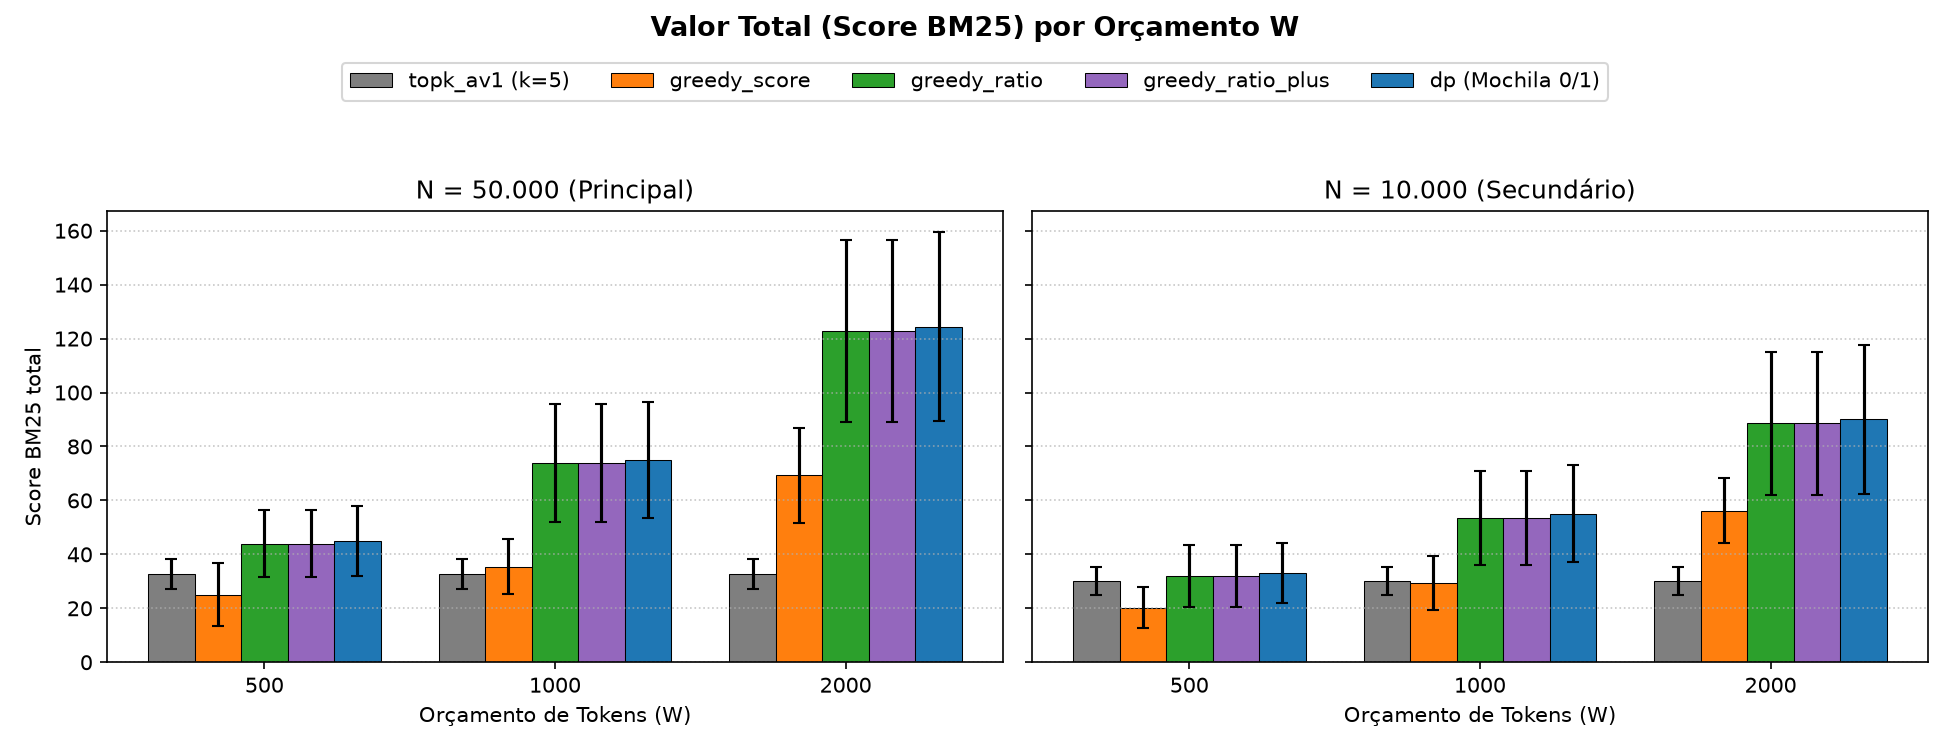
\includegraphics[width=0.75\textwidth]{av2_valor_total.png} \\ \vspace{0.2cm}
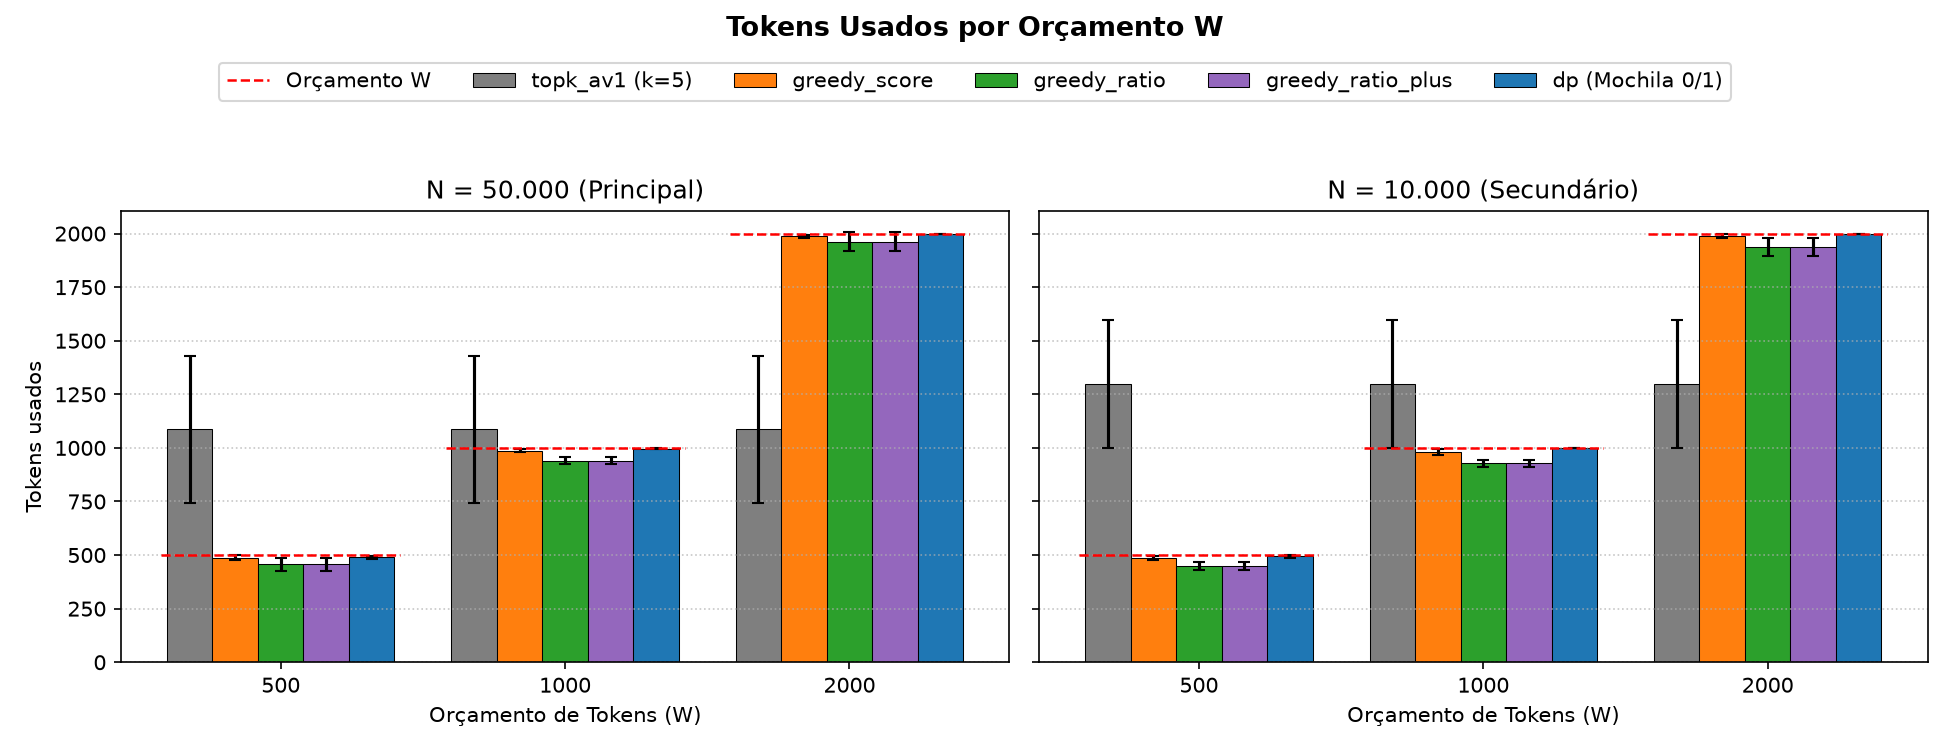
\includegraphics[width=0.75\textwidth]{av2_tokens_usados.png} \\ \vspace{0.2cm}
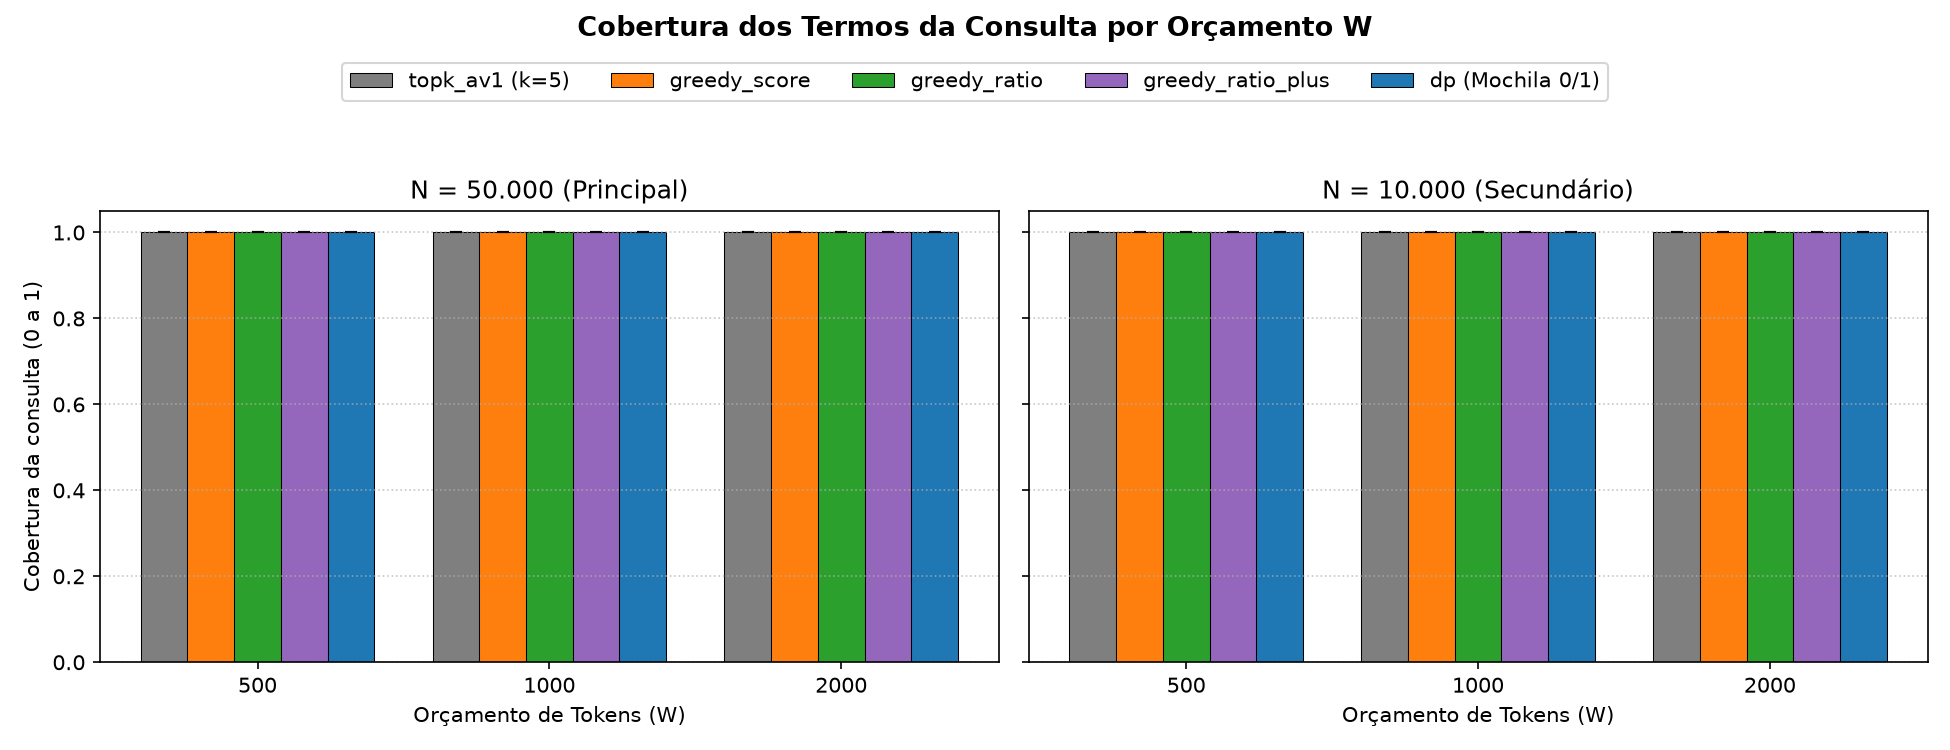
\includegraphics[width=0.75\textwidth]{av2_cobertura.png} \\ \vspace{0.2cm}
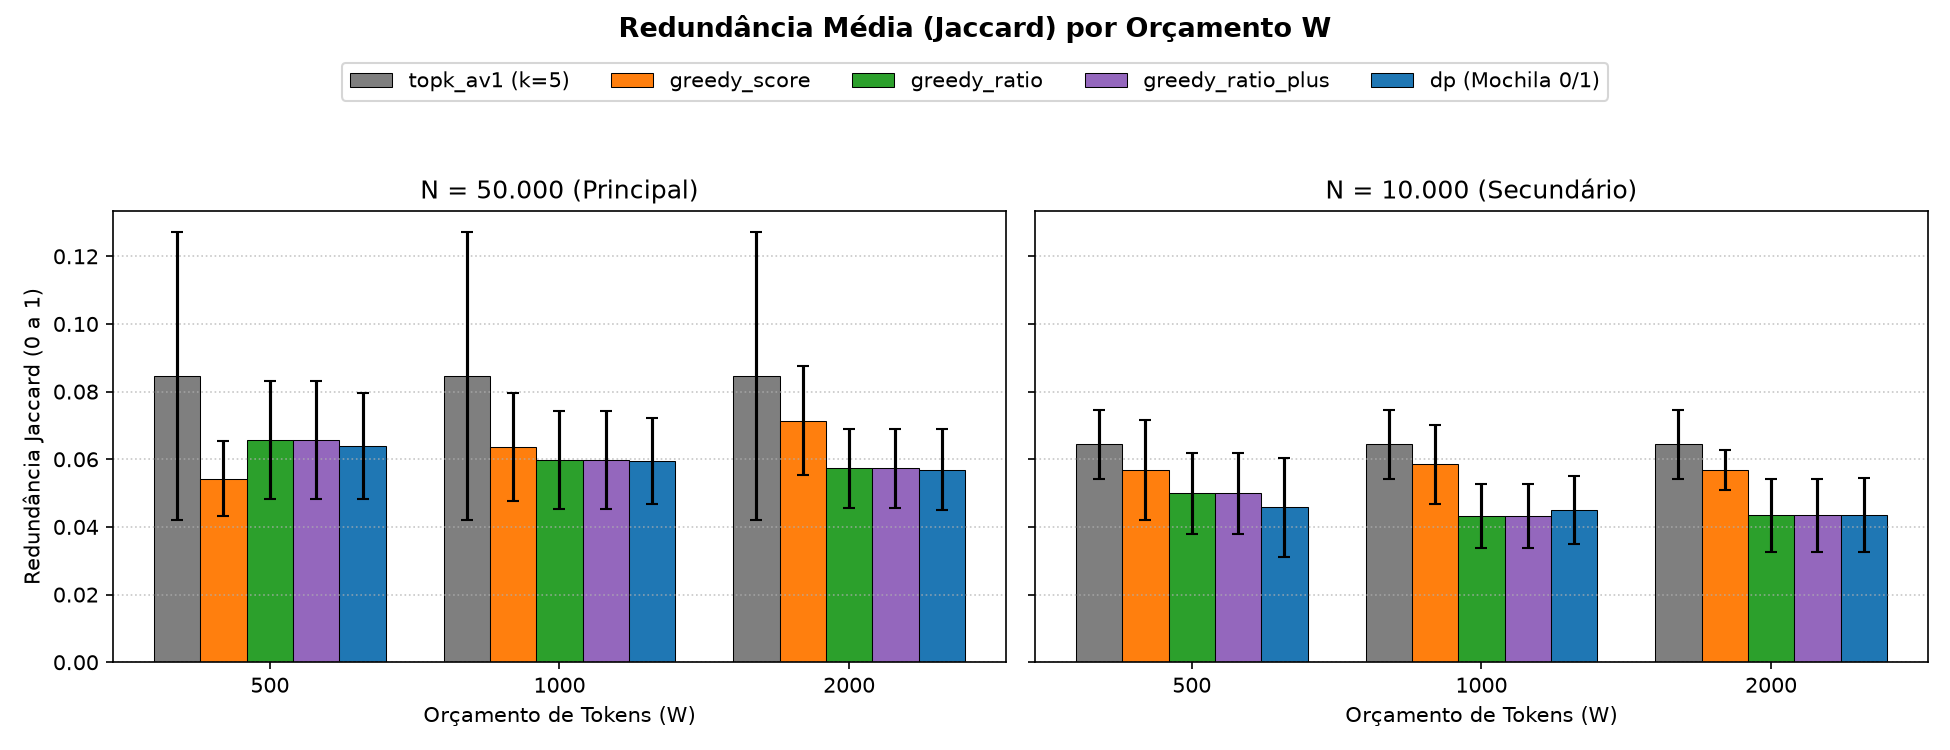
\includegraphics[width=0.75\textwidth]{av2_redundancia.png} \\ \vspace{0.2cm}
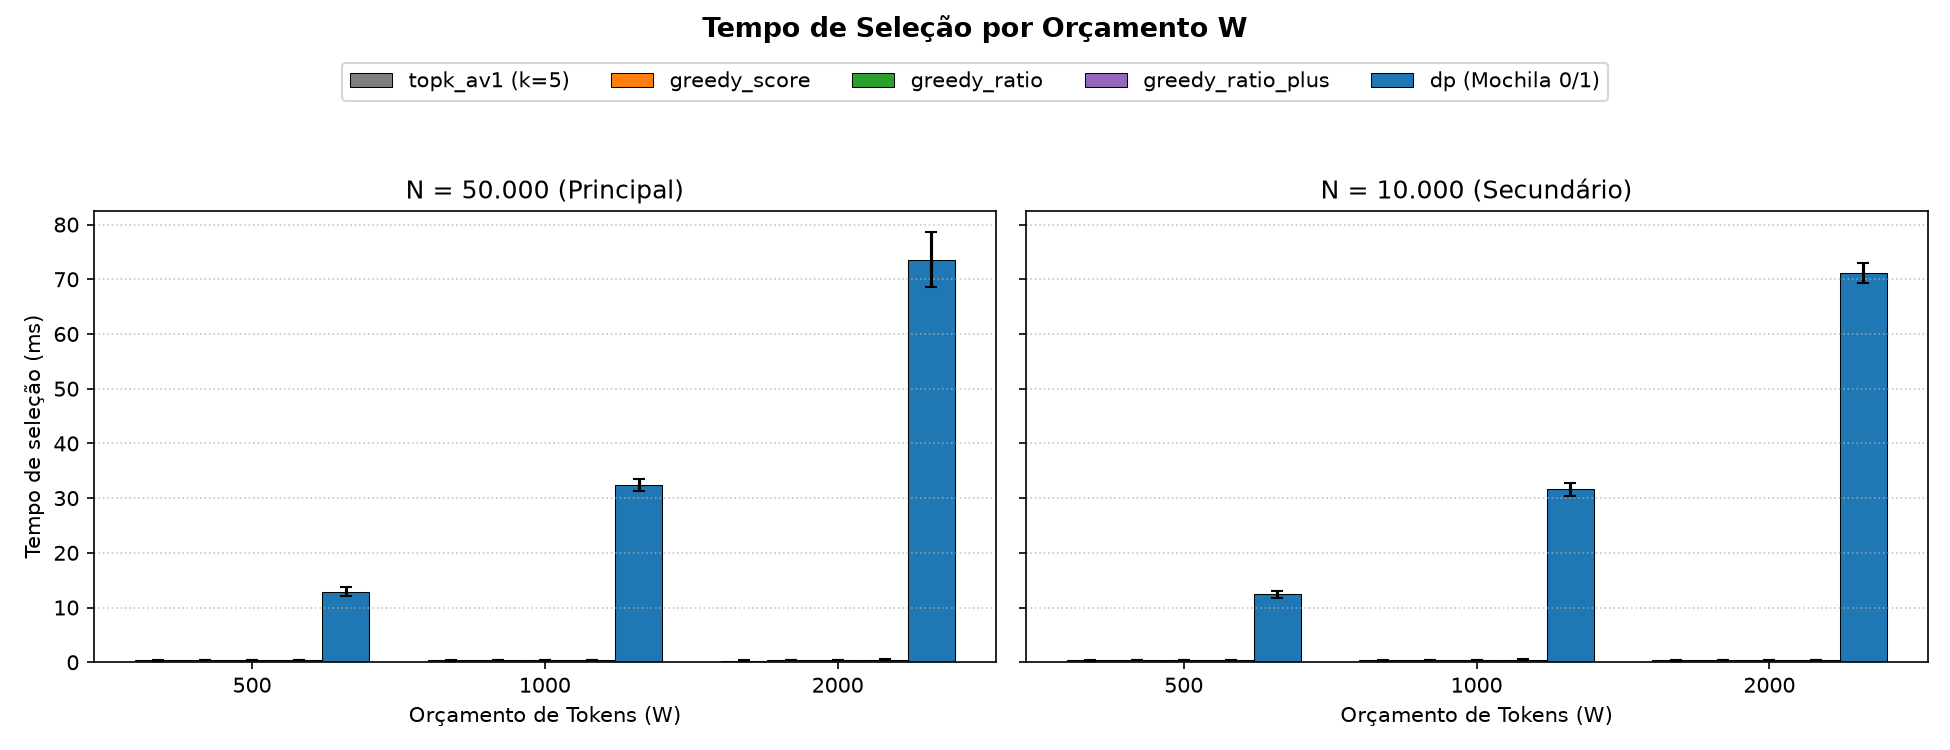
\includegraphics[width=0.75\textwidth]{av2_tempo_selecao.png}
\caption{Métricas consolidadas. O algoritmo exato (DP) otimiza o valor total respeitando o orçamento rigorosamente, enquanto a linha de base o ultrapassa.}
\label{fig:av2_graficos_consolidados}
\end{figure}

\subsection{Avaliação Manual de Relevância e Verificação (Testes)}
Na validação de controle (\texttt{av2\_validacao.csv}), a Programação Dinâmica (DP) obteve 100\% de concordância com a força bruta. Uma avaliação manual simples de Precision@k ($W=500$) confirmou trocas semânticas vantajosas: o algoritmo descarta arquivos muito extensos no topo por múltiplos textos mais concisos (média de 150 tokens) de alta pertinência, limitando o risco de \textit{truncation}.

A Tabela~\ref{tab:testes_av2} documenta o rastreamento dos casos de teste exigidos na especificação.

\begin{table}[H]
\centering
\footnotesize
\caption{Matriz de evidências e verificação de testes automatizados (AV2).}
\label{tab:testes_av2}
\begin{tabular}{cp{3.3cm}p{2.3cm}p{2.3cm}p{2.3cm}c}
\hline
\textbf{ID} & \textbf{Requisito Avaliado} & \textbf{Esperado} & \textbf{Observado} & \textbf{Evidência} & \textbf{Status} \\
\hline
T01 & DP em limites normais & $\le W$ e valor ótimo & Valores idênticos & Logs \texttt{pytest} & Passou \\
T02 & DP vs. Guloso adversarial & $\text{DP} > \text{Guloso}$ & $\text{DP}=13{,}0 > \text{Gul}=12{,}0$ & Logs \texttt{pytest} & Passou \\
T03 & Heurísticas de ratio/score& Respeito a $W$ & Orçamento válido & Logs \texttt{pytest} & Passou \\
T04 & Garantia do ratio\_plus & $V \ge 0{,}5 \cdot V_{opt}$ & Regra satisfeita & Logs \texttt{pytest} & Passou \\
T05 & Candidatos do baseline & $M$ itens ordenados & Estrutura íntegra & Logs \texttt{pytest} & Passou \\
T06 & DP igual Força Bruta & Delta $\le 10^{-9}$ & Diferença zero & Logs \texttt{pytest} & Passou \\
T07 & Métricas p4 (budget OK) & $\text{cov}=1{,}0, \text{ok}=V$ & Valores exatos & Logs \texttt{pytest} & Passou \\
T08 & Estouro/seleção vazia & $\text{cov}=0{,}0, \text{ok}=F$ & Valores exatos & Logs \texttt{pytest} & Passou \\
T09 & Pipeline integrado & Execução limpa & CSV gerado & \texttt{runs.csv} & Passou \\
T10 & Escalabilidade $M=200$ & Tolerância $W$ e OOM & Limites intactos & \texttt{runs.csv} & Passou \\
\hline
\end{tabular}
\end{table}

\subsection{Uso de IA neste pacote}
Modelos de IA generativa atuaram de forma restrita no mapeamento das fórmulas em \LaTeX{} e na compactação tabular. A conceção lógica das métricas de Jaccard no \texttt{src/metrics.py} e os julgamentos sobre violações de orçamento mantiveram-se sob análise da equipe.
\section{Relação com IA generativa, limitações e conclusão}

\subsection{Onde a seleção entra no RAG}
Em um sistema de geração aumentada por recuperação (RAG)~\cite{lewis2020}, o retriever devolve documentos candidatos e o prompt do modelo precisa caber em uma janela de contexto limitada. O problema estudado neste trabalho fica entre essas duas etapas: dados os $m = 200$ candidatos ordenados pelo BM25~\cite{robertson2009}, escolher quais deles vão para a janela. A escolha é um problema da mochila 0/1~\cite{kellerer2004}: cada documento tem valor (score BM25) e custo (tokens), e o orçamento $W$ é o limite de tokens reservado ao contexto.

O resultado da seleção afeta o sistema em três pontos:
\begin{itemize}
  \item \textbf{Tokens do prompt.} Com a seleção por mochila, o custo total nunca passa de $W$. O baseline da AV1, que envia os $k$ primeiros documentos, ignora $W$: na instância de teste F4 ele envia 11 tokens com $W = 4$.
  \item \textbf{Latência e custo.} A seleção ocorre antes da geração. O DP custa $\Theta(n \cdot W)$ em tempo e espaço, e os gulosos custam $\Theta(n \log n)$ pelo \emph{merge sort}~\cite{cormen2012}. Os tempos medidos por método, $N$ e $W$ estão na seção de resultados (rodada de 28/10).
  \item \textbf{Fundamentação da resposta.} O contexto escolhido limita o que o modelo pode citar. A seleção não verifica se a resposta gerada é fiel aos documentos: este protótipo não gera resposta, então não há verificação de afirmações.
\end{itemize}

\subsection{Riscos}
\begin{itemize}
  \item \textbf{Perder evidência relevante.} O DP maximiza a soma dos scores, não a qualidade de cada documento. Na instância F9 ($W = 10$), o DP escolhe três documentos de scores 3,0, 3,0 e 3,1 (soma 9,1) e descarta o documento de score 9,0, que sozinho ocupa todo o orçamento. O ganho em valor total é de 0,1, e o documento mais relevante fica fora do contexto.
  \item \textbf{Contexto enviesado.} Os scores vêm de um modelo apenas lexical sobre uma única fonte. Nenhuma das regras de seleção trata redundância ou diversidade, que são medidas à parte (cobertura e redundância).
  \item \textbf{Aproximação apresentada como ótimo.} As regras gulosas por score e por razão não têm garantia: na instância F1, a regra por razão escolhe valor 2,0 onde o ótimo é 10,0. Só a variante \texttt{ratio\_plus} garante pelo menos metade do valor ótimo. Os resultados devem dizer qual método foi usado.
\end{itemize}

\subsection{Limitações}
\begin{itemize}
  \item Fonte única de notícias (Folha de S.Paulo, 2015 a 2017).
  \item BM25 é apenas lexical e sofre com sinônimos e polissemia.
  \item O número de tokens é um proxy do custo real, que depende do tokenizador do modelo.
  \item O corte em $M = 200$ candidatos pode deixar de fora documentos úteis.
  \item Apenas três valores de orçamento: $W \in \{500, 1000, 2000\}$.
  \item Todas as medições vêm de Python em uma única máquina, sem paralelismo.
\end{itemize}

\subsection{Conclusão}
A mochila 0/1 resolvida por programação dinâmica é a única das regras testadas que garante um contexto ótimo dentro do orçamento de tokens, ao custo de $\Theta(n \cdot W)$. Os gulosos são mais rápidos, mas só a variante \texttt{ratio\_plus} tem garantia, de 1/2 do ótimo. O ganho medido do DP sobre os gulosos e sobre o top-5 da AV1 está na seção de resultados. Vídeo de apresentação: \url{https://youtu.be/JimsN27pCZA}.

\subsection*{Uso de IA neste pacote}
\begin{itemize}
  \item Ferramenta e modelo: Claude (Anthropic), modelo Sonnet 5.5.
  \item Finalidade: escrever o programa \texttt{experiments/run\_av2.py}, os testes T09 e T10, o README, a licença e as seções e slides do pacote 5.
  \item Prompts relevantes (até 5): implementar o pacote 5 do plano da AV2; escrever a seção \texttt{p5.tex} e os slides conforme o plano.
  \item Sugestões aproveitadas, corrigidas ou rejeitadas: a estrutura do plano foi seguida; o conteúdo dos slides sugerido inicialmente foi corrigido para o que o plano pede (relação com RAG, limitações e conclusão).
  \item Erros identificados e como foram verificados: os exemplos numéricos (F1, F4 e F9) foram conferidos contra as instâncias fixas do plano; os testes T09 e T10 foram executados.
\end{itemize}

\begin{thebibliography}{9}
\bibitem{cormen2012} Cormen, T. H.; Leiserson, C. E.; Rivest, R. L.; Stein, C. \emph{Algoritmos: Teoria e Prática}. 3.\ ed. Rio de Janeiro: Elsevier, 2012.
\bibitem{kellerer2004} Kellerer, H.; Pferschy, U.; Pisinger, D. \emph{Knapsack Problems}. Berlim: Springer, 2004.
\bibitem{robertson2009} Robertson, S.; Zaragoza, H. The Probabilistic Relevance Framework: BM25 and Beyond. \emph{Foundations and Trends in Information Retrieval}, v. 3, n. 4, p. 333--389, 2009.
\bibitem{lewis2020} Lewis, P. et al. Retrieval-Augmented Generation for Knowledge-Intensive NLP Tasks. In: \emph{Advances in Neural Information Processing Systems}, v. 33, 2020.
\end{thebibliography}


\end{document}